\documentclass{article}

% 导入中文宏包
\usepackage{ctex}
\usepackage{array}
\usepackage{caption}
\usepackage{hyperref}
% 设置页面边距
\usepackage{geometry}
\usepackage{graphicx}
\geometry{a4paper, left=2.5cm, right=2.5cm, top=3cm, bottom=3cm}

% 设置标题、作者和日期
\title{Shell和Vim}
\author{23020007030  关嘉琪}

\begin{document}
	
	% 生成标题、作者和日期
	\maketitle
	
	% 心得报告正文
	\section{实验目的}
	本次课程主要讲授了Shell工具和脚本,用编辑器Vim进行数据整理。
	
	\section{介绍}
	\subsection{两大工具的优点}
	Shell是系统的用户界面,提供了用户与内核进行交互操作的一种接口。它接收用户输入的命令并把它送入内核去执行。实际上Shell是一个命令解释器,它解释由用户输入的命令并且把它们送到内核。不仅如此,Shell有自己的编程语言用于对命令的编辑,它允许用户编写由shell命令组成的程序。Shell编程语言具有普通编程语言的很多特点,比如它也有循环结构和分支控制结构等,用这种编程语言编写的Shell程序与其他应用程序具有同样的效果。
	
	Vim是从vi发展出来的一个文本编辑器。代码补全、编译及错误跳转等方便编程的功能特别丰富,在程序员中被广泛使用,和Emacs并列成为类Unix系统用户最喜欢的文本编辑器。vim的设计理念是命令的组合。用户学习了各种各样的文本间移动/跳转的命令和其他的普通模式的编辑命令,并且能够灵活组合使用的话,能够比那些没有模式的编辑器更加高效的进行文本编辑。同时VIM与很多快捷键设置和正则表达式类似,可以辅助记忆。并且vim针对程序员做了优化。
	\section{实验内容}
	\subsection{Shell学习例子10个}
	
	1.echo "Hello, World!"
	
	用Shell打印hello world
	echo 是一个在命令行界面(shell)中常用的命令,
	它的主要作用是输出(显示)一段文本或者变量的值到标准输出
	
	\noindent
	\begin{minipage}{\linewidth}
		\centering
		% 插入图片
		
\includegraphics[width=0.5\linewidth]{example1.png}
		% 图片标题
		\captionof{figure}{echo 用来显示文本或变量}
		\label{fig:example}
	\end{minipage}
	
	
	2.变量赋值以及变量的使用
	\begin{verbatim}
		word="Hello, Git Bash!"
		echo $word
		#向word变量赋值,再通过echo $输出变量
	\end{verbatim}
	
	
	\noindent
	\begin{minipage}{\linewidth}
		\centering
		% 插入图片
		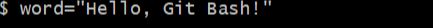
\includegraphics[width=0.5\linewidth]{example2.1.png}
		% 图片标题
	\end{minipage}
	\noindent
	\begin{minipage}{\linewidth}
		\centering
		% 插入图片
		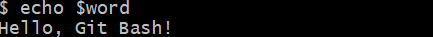
\includegraphics[width=0.5\linewidth]{example2.2.png}
		\captionof{figure}{变量的赋值和使用}
		\label{fig:example}
	\end{minipage}
	
	
	3.条件语句
	\begin{verbatim}
		if [ "$word" = "Hello, Git Bash!" ];then
		echo "Yes."
		else
		echo "No."
		fi
		#[]里是条件判断,then后面是条件正确的结果,else是条件错误的结果
		
	\end{verbatim}
	
	\noindent
	\begin{minipage}{\linewidth}
		\centering
		% 插入图片
		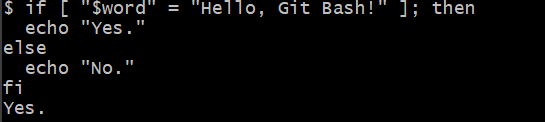
\includegraphics[width=0.5\linewidth]{example3.png}
		% 图片标题
		\captionof{figure}{条件语句的判断}
		\label{fig:example}
	\end{minipage}
	
	4.循环语句
	\begin{verbatim}
		for i in {1..5}; do
		echo "number: $i"
		done
		#in {1..5} 指定了循环的范围。
		在这个例子中,{1..5} 是一个序列表达式,表示从1到5的数字序列,包括1和5。
		done是结束这个循环
	\end{verbatim}
	
	\noindent
	\begin{minipage}{\linewidth}
		\centering
		% 插入图片
		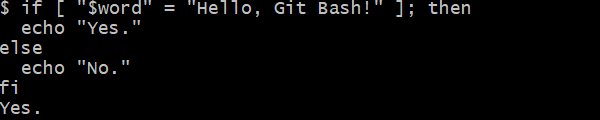
\includegraphics[width=0.5\linewidth]{example4.1.png}
	\end{minipage}
	\noindent
	\begin{minipage}{\linewidth}
		\centering
		% 插入图片
		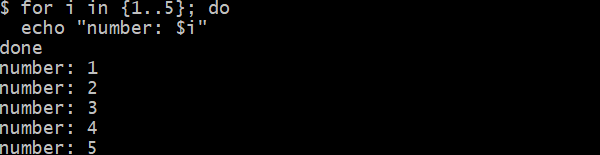
\includegraphics[width=0.5\linewidth]{example4.2.png}
		% 图片标题
		\captionof{figure}{循环语句}
		\label{fig:example}
	\end{minipage}
	
	5.文件的建立与写入
	\begin{verbatim}
		创建一个新文件
		touch example.txt
		
		写入内容到文件
		echo "This is an example file." > example.txt
		
		读取文件内容
		cat example.txt     
	\end{verbatim}
	
	
	\noindent
	\begin{minipage}{\linewidth}
		\centering
		% 插入图片
		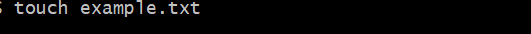
\includegraphics[width=0.5\linewidth]{example5.1.png}
	\end{minipage}
	\noindent
	\begin{minipage}{\linewidth}
		\centering
		% 插入图片
		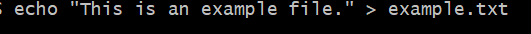
\includegraphics[width=0.5\linewidth]{example5.2.png}
	\end{minipage}
	\noindent
	\begin{minipage}{\linewidth}
		\centering
		% 插入图片
		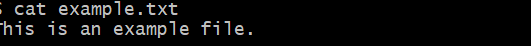
\includegraphics[width=0.5\linewidth]{example5.3.png}
		% 图片标题
		\captionof{figure}{创建写入读取文件}
		\label{fig:example}
	\end{minipage}
	
	6.创建目录与切换
	\begin{verbatim}
		创建一个新目录
		mkdir new_directory
		切换到新目录
		cd new_directory
	\end{verbatim}
	
	
	
	\noindent
	\begin{minipage}{\linewidth}
		\centering
		% 插入图片
		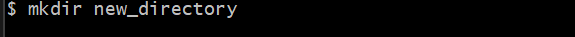
\includegraphics[width=0.5\linewidth]{example6.1.png}
	\end{minipage}
	\noindent
	\begin{minipage}{\linewidth}
		\centering
		% 插入图片
		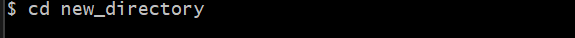
\includegraphics[width=0.5\linewidth]{example6.2.png}
		% 图片标题
		\captionof{figure}{创建与切换新目录}
		\label{fig:example}
	\end{minipage}
	
	7.函数的创建和使用
	\begin{verbatim}
		greet() {
			echo "Hello, $1!"
		}
		
		greet "Shell"
		
	\end{verbatim}
	
	\noindent
	\begin{minipage}{\linewidth}
		\centering
		% 插入图片
		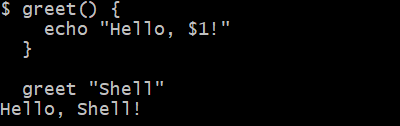
\includegraphics[width=0.5\linewidth]{example7.png}
		% 图片标题
		\captionof{figure}{定义函数与使用}
		\label{fig:example}
	\end{minipage}
	
	8.加法运算
	\begin{verbatim}
		a=5
		b=7
		sum=$(($a + $b))
		echo "The sum of $a and$b is: $sum"
	\end{verbatim}
	
	
	
	\noindent
	\begin{minipage}{\linewidth}
		\centering
		% 插入图片
		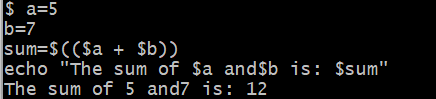
\includegraphics[width=0.5\linewidth]{example8.png}
		% 图片标题
		\captionof{figure}{进行加法运算}
		\label{fig:example}
	\end{minipage}
	
	9. 获取工作目录,并列出工作目录
	\begin{verbatim}
		# 获取当前工作目录
		pwd
		# 列出当前目录下的所有文件和目录
		ls -l
	\end{verbatim}
	
	\noindent
	\begin{minipage}{\linewidth}
		\centering
		% 插入图片
		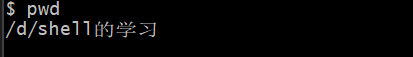
\includegraphics[width=0.5\linewidth]{example9.1.png}
	\end{minipage}
	\noindent
	\begin{minipage}{\linewidth}
		\centering
		% 插入图片
		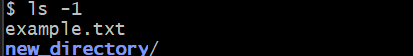
\includegraphics[width=0.5\linewidth]{example9.2.png}
		% 图片标题
		\captionof{figure}{获取目录并列出当前目录}
		\label{fig:example}
	\end{minipage}
	
	10.查看当前目录文件数目
	\begin{verbatim}
		file_count=$(ls -1 | wc -l)
		echo "There are $file_count files in the current directory."
	\end{verbatim}
	
	
	\noindent
	\begin{minipage}{\linewidth}
		\centering
		% 插入图片
		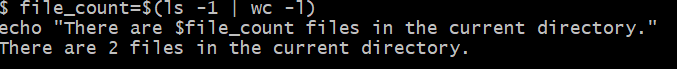
\includegraphics[width=0.5\linewidth]{example10.png}
		% 图片标题
		\captionof{figure}{查看当前目录文件数目}
		\label{fig:example}
	\end{minipage}
	
	
	
	\subsection{Vim学习例子10个}
	1.Vim文件的创立,
	在终端中输入 vim example.txt
	
	
	\noindent
	\begin{minipage}{\linewidth}
		\centering
		% 插入图片
		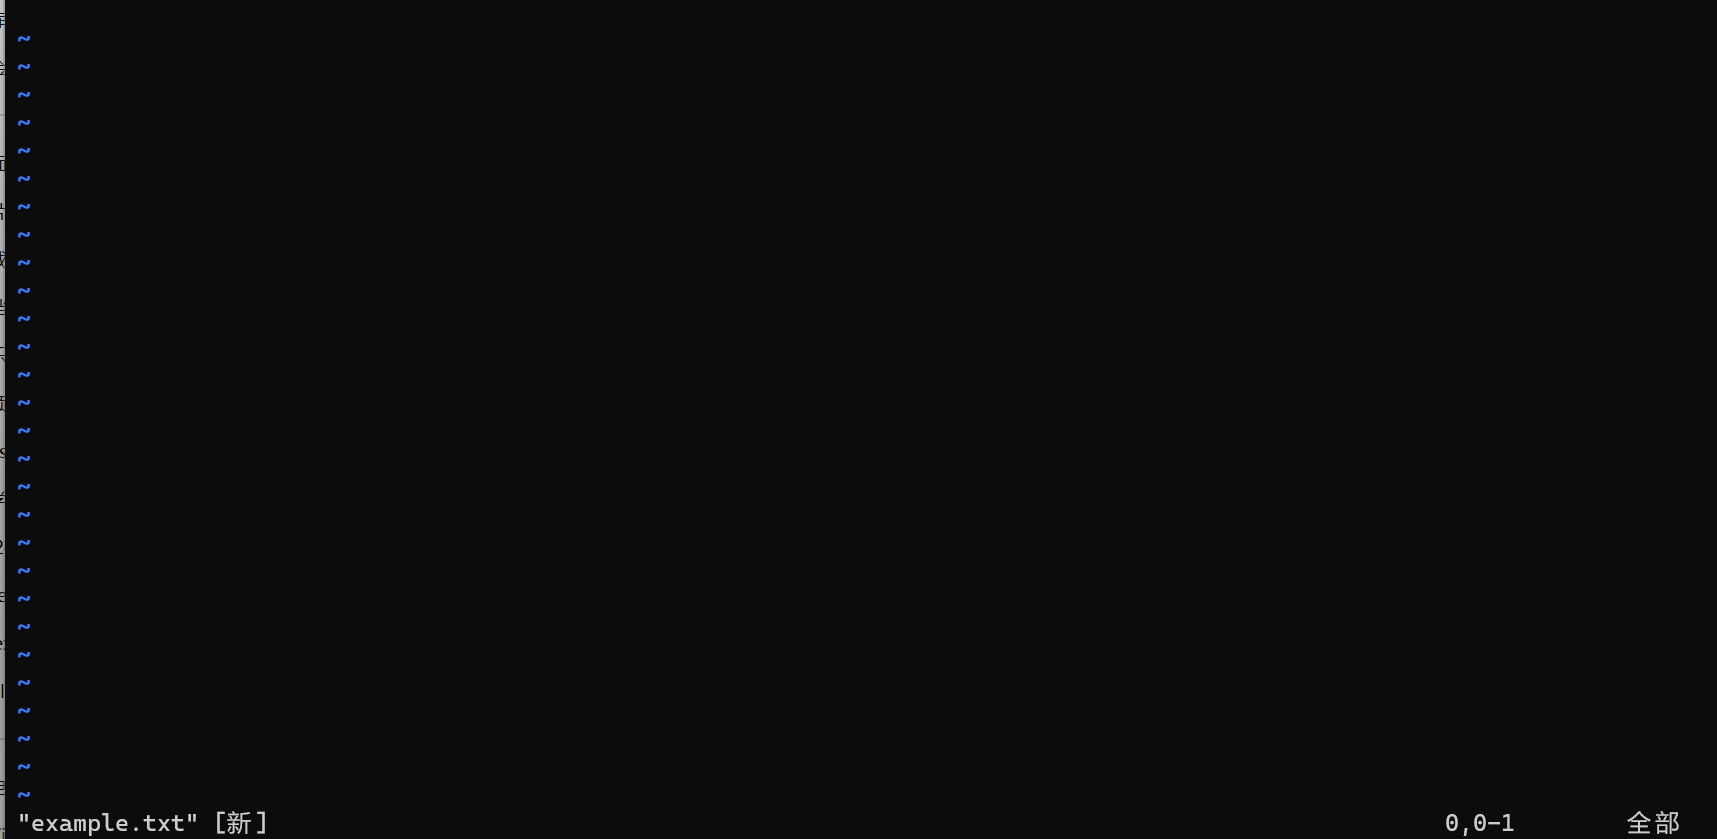
\includegraphics[width=0.5\linewidth]{example11.png}
		% 图片标题
		\captionof{figure}{Vim文件的创立}
		\label{fig:example}
	\end{minipage}
	
	2. i键为插入,开始输入内容hello,vim!
	
	\noindent
	\begin{minipage}{\linewidth}
		\centering
		% 插入图片
		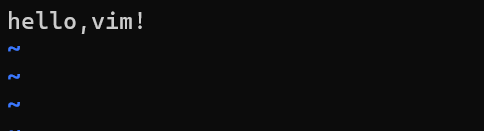
\includegraphics[width=0.5\linewidth]{example12.png}
		% 图片标题
		\captionof{figure}{i插入内容}
		\label{fig:example}
	\end{minipage}
	
	3.编辑的退出与保存
	\begin{verbatim}
		Esc是回到正常模式
		:w带编者保存
		:q代表退出
		如果不按w的话则文件为SWP文件,用于临时储存数据
	\end{verbatim}
	
	\noindent
	\begin{minipage}{\linewidth}
		\centering
		% 插入图片
		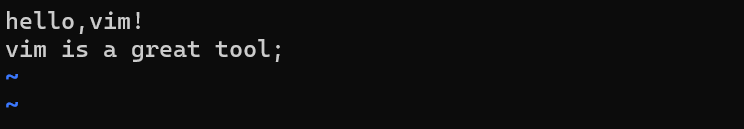
\includegraphics[width=0.5\linewidth]{example13.png}
		% 图片标题
		\captionof{figure}{编辑的退出与保存}
		\label{fig:example}
	\end{minipage}
	
	
	
	4.dd表示删除当前行
	\begin{verbatim}
		在vim is a greet tool前输入dd删除后的结果
	\end{verbatim}
	
	
	\noindent
	\begin{minipage}{\linewidth}
		\centering
		% 插入图片
		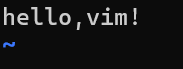
\includegraphics[width=0.5\linewidth]{example14.png}
		% 图片标题
		\captionof{figure}{dd删除当前行后的结果}
		\label{fig:example}
	\end{minipage}
	
	5.dw:删除光标后的单词。
	
	\noindent
	\begin{minipage}{\linewidth}
		\centering
		% 插入图片
		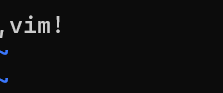
\includegraphics[width=0.5\linewidth]{example15.png}
		% 图片标题
		\captionof{figure}{dw删除光标后的单词的结果}
		\label{fig:example}
	\end{minipage}
	
	6.x:删除光标下的字符。
	
	\noindent
	\begin{minipage}{\linewidth}
		\centering
		% 插入图片
		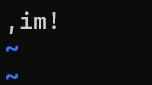
\includegraphics[width=0.5\linewidth]{example16.png}
		% 图片标题
		\captionof{figure}{删除光标下的字符的结果}
		\label{fig:example}
	\end{minipage}
	
	7.r:替换光标下的单个字符。
	R:进入替换模式,连续替换多个字符直到按下 Esc。
	
	
	\noindent
	\begin{minipage}{\linewidth}
		\centering
		% 插入图片
		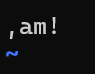
\includegraphics[width=0.5\linewidth]{example17.png}
		% 图片标题
		\captionof{figure}{用r替换光标下的单个字符}
		\label{fig:example}
	\end{minipage}
	
	\noindent
	\begin{minipage}{\linewidth}
		\centering
		% 插入图片
		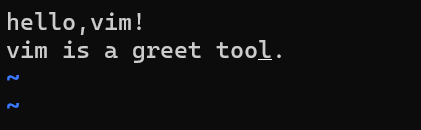
\includegraphics[width=0.5\linewidth]{example18.png}
		% 图片标题
		\captionof{figure}{在R模式未改变前}
		\label{fig:example}
	\end{minipage}
	
	\noindent
	\begin{minipage}{\linewidth}
		\centering
		% 插入图片
		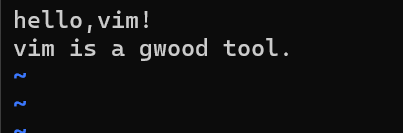
\includegraphics[width=0.5\linewidth]{example19.png}
		% 图片标题
		\captionof{figure}{在R模式改变后}
		\label{fig:example}
	\end{minipage}
	
	8. 
	u:撤销最后一次更改。
	
	Ctrl + r:重做最后一次撤销,即反撤销。
	
	
	\begin{minipage}{\linewidth}
		\centering
		% 插入图片
		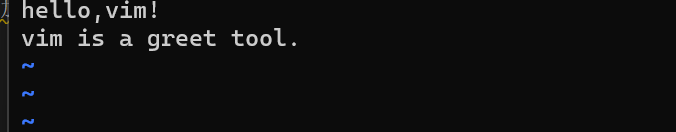
\includegraphics[width=0.5\linewidth]{example20.png}
		% 图片标题
		\captionof{figure}{撤销}
		\label{fig:example}
	\end{minipage}
	
	\begin{minipage}{\linewidth}
		\centering
		% 插入图片
		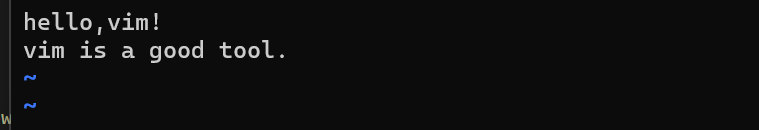
\includegraphics[width=0.5\linewidth]{example21.png}
		% 图片标题
		\captionof{figure}{反撤销}
		\label{fig:example}
	\end{minipage}
	
	
	9.复制的学习:
	
	复制单行:
	将光标移动到要复制的行的任意位置。
	输入 yy 来复制整行。
	
	复制部分行:
	将光标移动到要开始复制的位置。
	进入可视化模式,可以按 v(用于字符模式)或 V(用于行模式)。
	使用光标键hjkl选择要复制的文本。
	一旦选择了文本,按 y 来复制选中的文本。
	
	复制多个行:
	将光标移动到要复制的第一行的任意位置。
	输入 数字yy,其中 “数字” 是您想要复制的行数。
	例如,3yy 会复制光标所在的当前行以及下面两行,总共三行。
	
	\noindent
	\begin{minipage}{\linewidth}
		\centering
		% 插入图片
		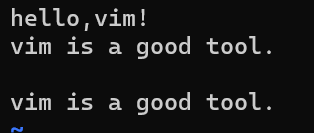
\includegraphics[width=0.5\linewidth]{example22.png}
		% 图片标题
		\captionof{figure}{复制一行后的结果}
		\label{fig:example}
	\end{minipage}
	
	\noindent
	\begin{minipage}{\linewidth}
		\centering
		% 插入图片
		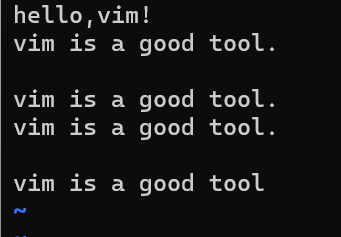
\includegraphics[width=0.5\linewidth]{example23.png}
		% 图片标题
		\captionof{figure}{选择性复制后的结果}
		\label{fig:example}
	\end{minipage}
	
	
	10.
	p:在光标后粘贴。
	P:在光标前粘贴。
	下面是粘贴后的结果
	
	\noindent
	\begin{minipage}{\linewidth}
		\centering
		% 插入图片
		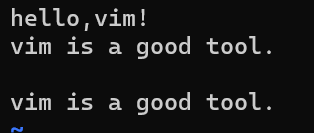
\includegraphics[width=0.5\linewidth]{example22.png}
		% 图片标题
		\captionof{figure}{粘贴后的结果}
		\label{fig:example}
	\end{minipage}
	
	
	
	
	\section{实验总结}
	Shell是一种强大的自动化工具。通过编写脚本,可以将日常繁琐的任务变得简单高效,这让我对编程产生了浓厚的兴趣,也锻炼了我的逻辑思维能力。
	与此同时,Shell的学习让我更加深入地理解了操作系统的内部工作原理,我开始意识到,每一个命令背后都隐藏着复杂而精巧的设计,这激发了我对技术的探索欲。
	
	Vim完全改变了我对文本编辑的看法。起初,Vim的模式系统和快捷键让我感到困惑,但随着时间的推移,熟练使用Vim后,我编辑文本的速度和准确性都有了显著提升。
	Vim的学习过程也是对个人习惯的一次挑战。它要求我放弃一些固有的操作习惯,转而接受一种更高效的工作方式。这个过程虽然艰难,但也让我认识到,改变习惯需要时间和耐心,而一旦新的习惯形成,它将带来巨大的收益。
	
	总的来说,Shell和Vim的学习不仅仅提升了我的技术能力,更让我在解决问题的思维方式上有了新的认识。
	
	github路径
	您可以在此查看项目的源代码: 
	
	\url{https://github.com/Joyceapple/repo/tree/a6610e40fed36fe130b1662340c80d2873dcdd7b/shell_vim}
\end{document}
